\documentclass[aspectratio=169]{beamer}
\usepackage{amsmath, amssymb, amsfonts, amsthm}
\usepackage{lmodern}
\usepackage{cancel}
\usepackage[output-complex-root=j]{siunitx}
\usepackage[american, nooldvoltagedirection]{circuitikz}
\usepackage{bm}
\usepackage{listings}
\usepackage{graphicx}
\usepackage{hyperref}

\usetheme{Berkeley}
\usefonttheme[onlymath]{serif}
\AtBeginSection[]{
    \begin{frame}
    \vfill
    \centering
    \begin{beamercolorbox}[sep=8pt,center,shadow=false,rounded=false]{title}
    \usebeamerfont{title}\insertsectionhead\par
    \end{beamercolorbox}
    \vfill
    \end{frame}
}

\newcommand{\N}{\mathbb{N}}
\newcommand{\Z}{\mathbb{Z}}
\newcommand{\Q}{\mathbb{Q}}
\newcommand{\R}{\mathbb{R}}
\renewcommand{\C}{\mathbb{C}}
\newcommand{\tpose}[1]{\left[#1\right]^{\! \top} \!\!}

\title{EECS 16B CSM}
\author{Bryan Ngo}
\date{2020-11-15}
\institute{UC Berkeley}

\begin{document}

\begin{frame}
    \maketitle
\end{frame}

\section{Principal Component Analysis}

\begin{frame}
    \frametitle{Motivation}

    \begin{itemize}
        \item used for statistical analysis
        \item clustering
        \item correlation
    \end{itemize}
\end{frame}

\begin{frame}
    \frametitle{How to PCA}

    Given \(\bm{A} \in \R^{n \times m}\), \(n\) measurements with \(m\) samples,
    \begin{enumerate}
        \item find \(\overline{n_i}\) to center \(\bm{A}\) around mean
        \item find covariance matrix \(\bm{C} = \frac{1}{m} \tpose{\widetilde{\bm{A}}} \widetilde{\bm{A}}\)
        \item plot any two eigenvectors/principal components \(v_1, v_2\) against centered points
        \item data is scaled by \(\sigma_1, \sigma_2\)
        \item more stretched along vector \(\implies\) larger correlation
    \end{enumerate}
\end{frame}

\begin{frame}
    \frametitle{Visualization}

    \centering
    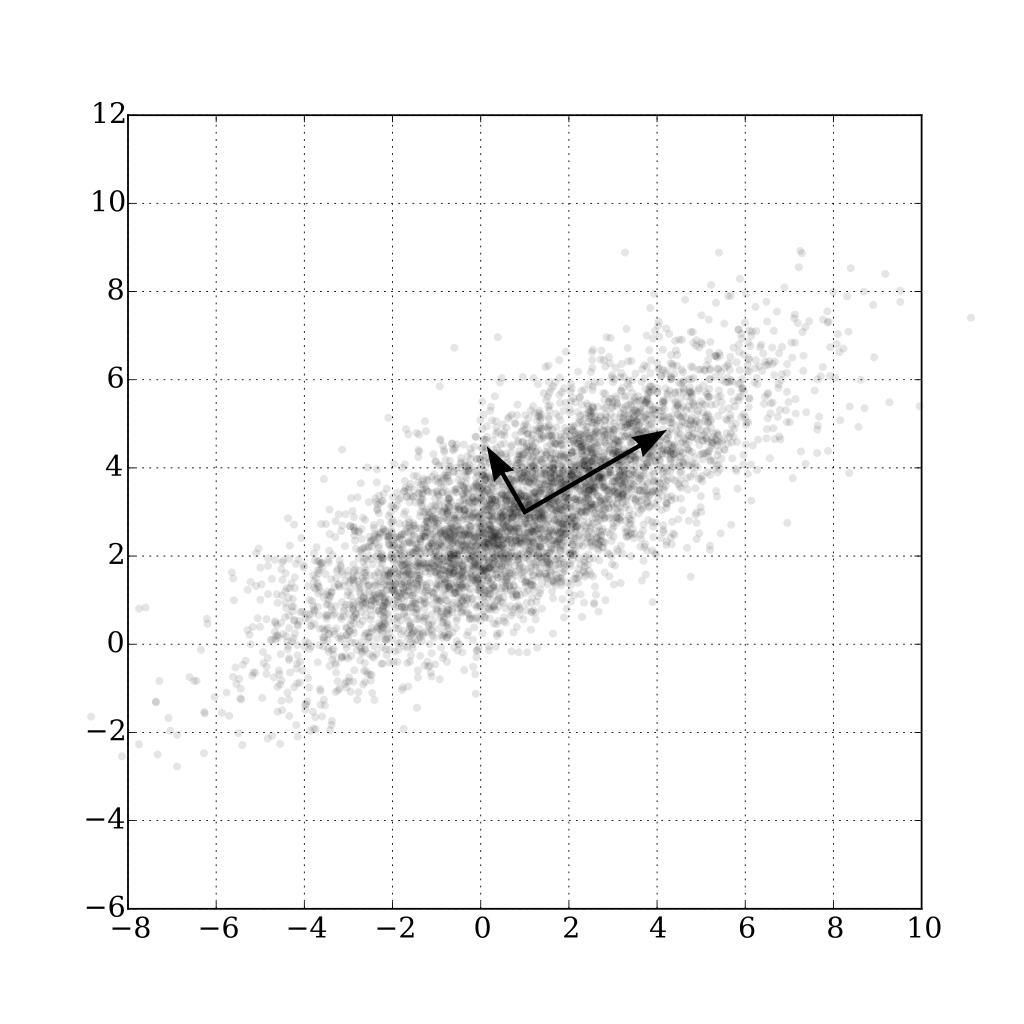
\includegraphics[height=0.9\textheight]{1024px-GaussianScatterPCA.svg.png}
\end{frame}

\section{Signals}

\begin{frame}
    \frametitle{Sampling}

    \begin{itemize}
        \item continuous \(\to\) discrete
        \item measuring an analog signal at a frequency \(\omega\)
        \item band limiting \begin{itemize}
            \item if \(\omega > 2 \omega_{max}\), signal perfectly recovered (Nyquist frequency)
        \end{itemize}
    \end{itemize}
\end{frame}

\begin{frame}
    \frametitle{Interpolation}

    \begin{itemize}
        \item discrete \(\to\) continuous
        \item we want to pass through every sampling point, not approximate it
        \item composed of a weighted sum of basis functions
    \end{itemize}
    Given basis function
    \begin{align}
        \Phi_i(x) &=
        \begin{cases}
            1 & x = i \\
            0 & \text{elsewhere}
        \end{cases} \\
        y(x) &= \sum_{i = 1}^n y_i \Phi_i(x)
    \end{align}
\end{frame}

\begin{frame}
    \frametitle{Interpolation}
    \framesubtitle{Zero-Hold}

    \centering
    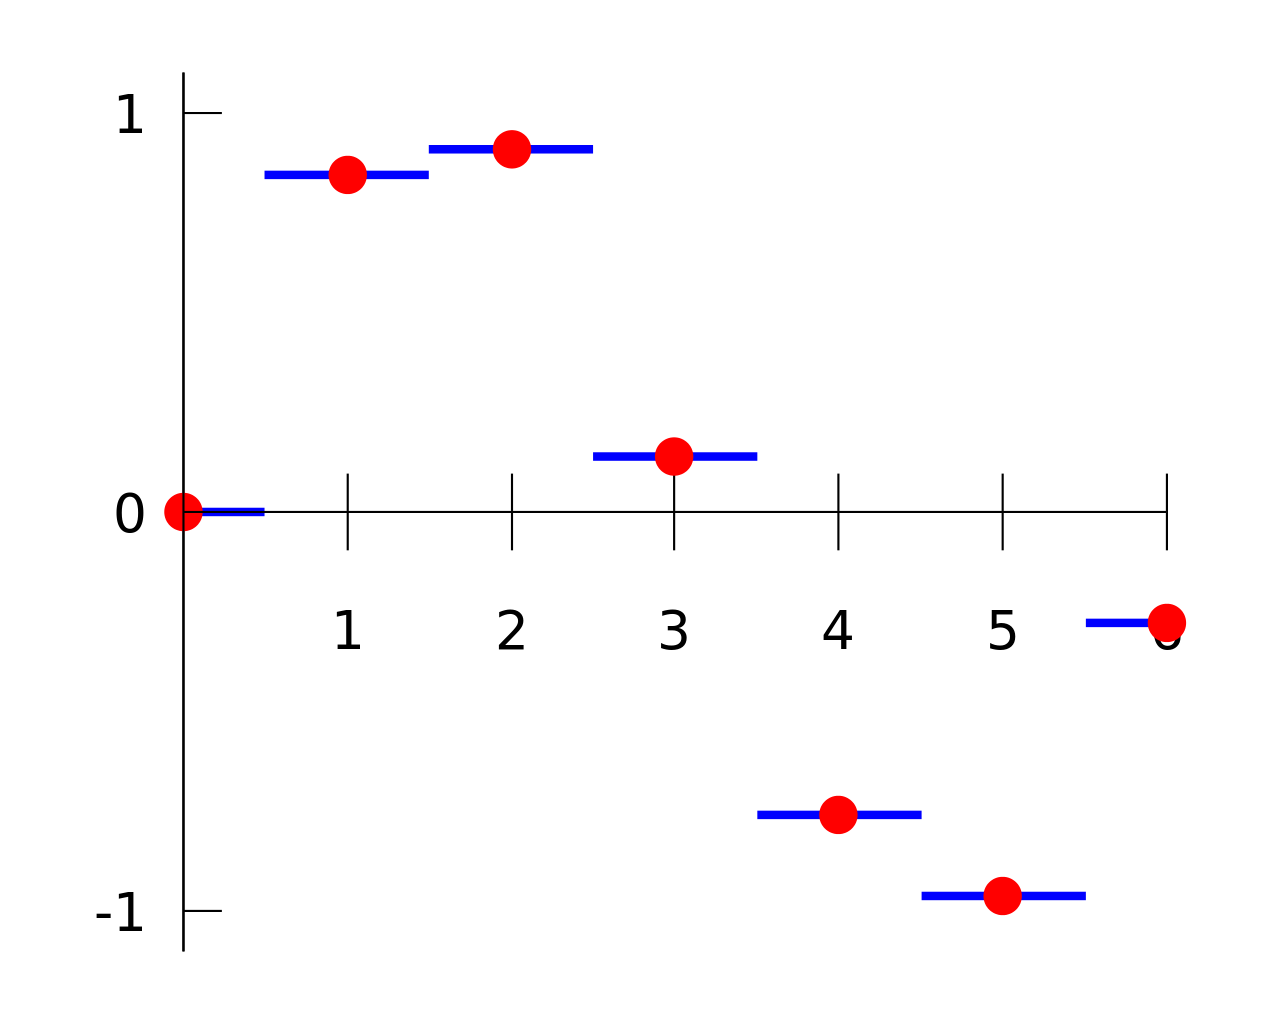
\includegraphics[height=0.9\textheight]{1280px-Piecewise_constant.svg.png}
\end{frame}

\begin{frame}
    \frametitle{Interpolation}
    \framesubtitle{Linear}

    \centering
    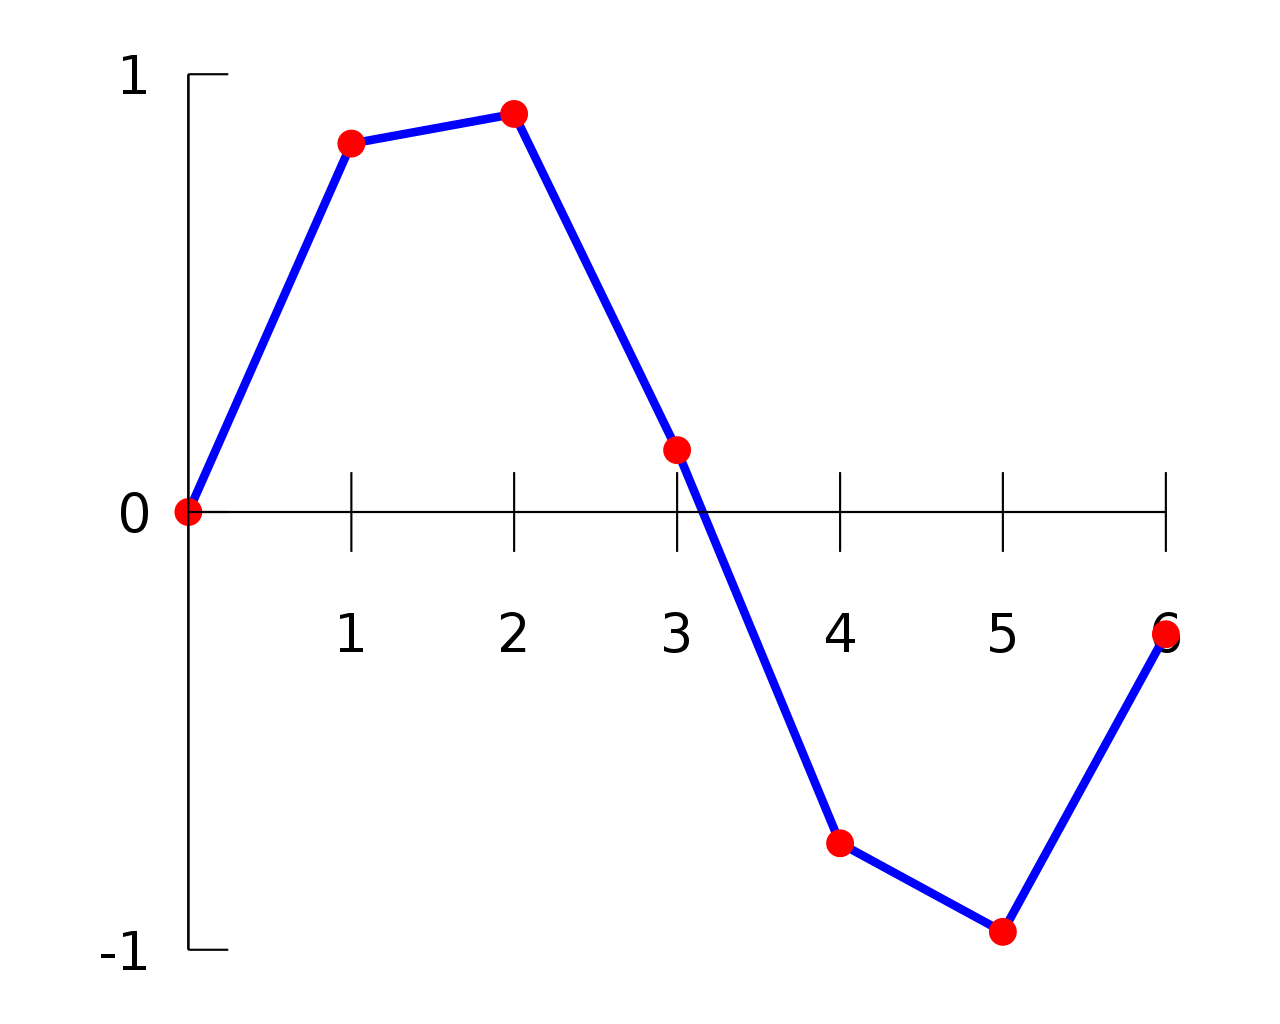
\includegraphics[height=0.9\textheight]{1280px-Interpolation_example_linear.svg.png}
\end{frame}

\begin{frame}
    \frametitle{Interpolation}
    \framesubtitle{Polynomial}

    \centering
    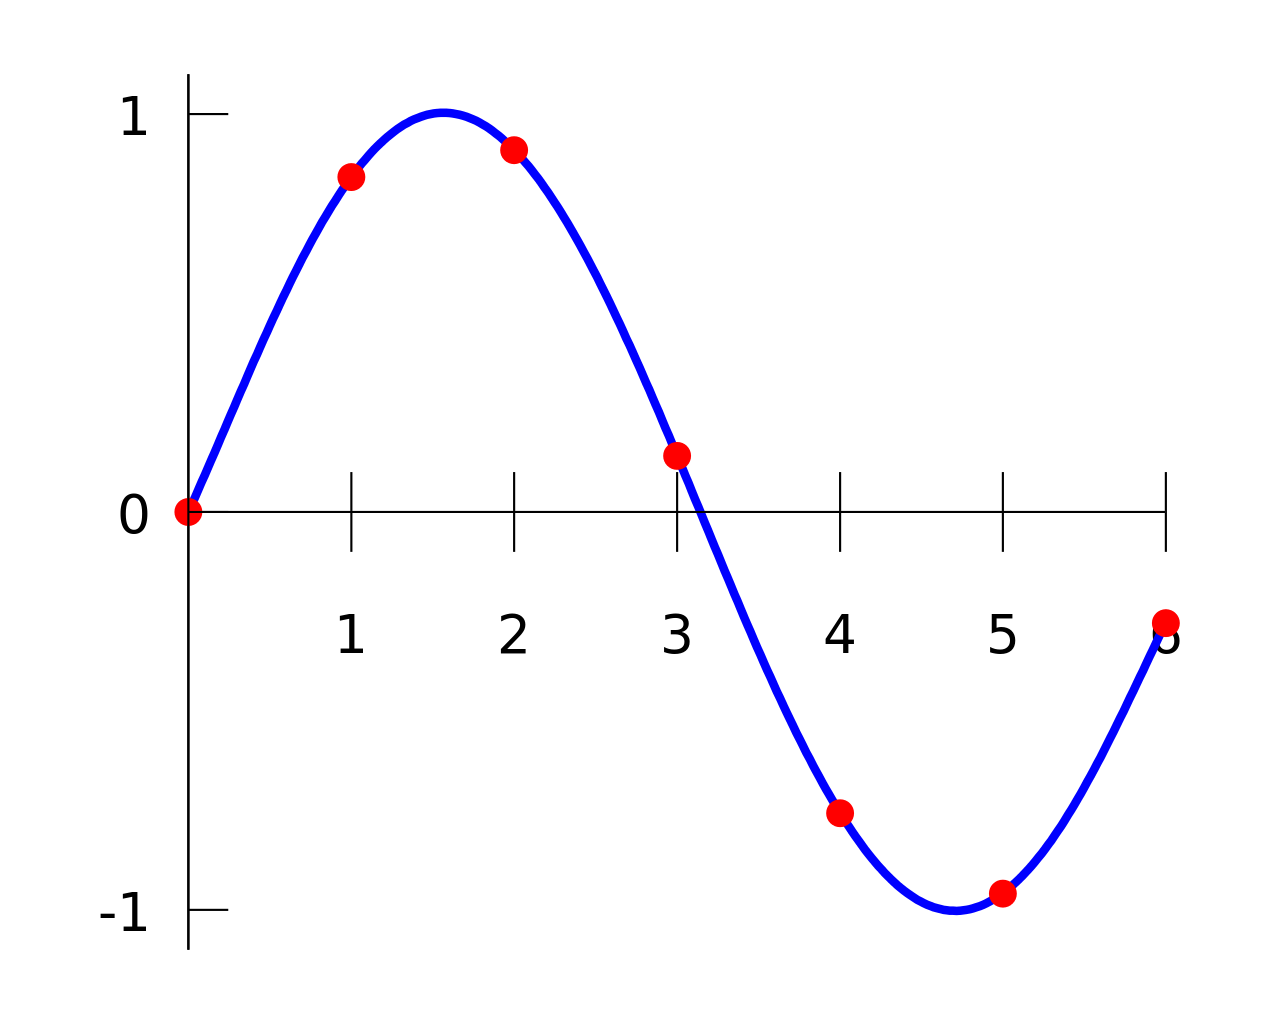
\includegraphics[height=0.9\textheight]{1280px-Interpolation_example_polynomial.svg.png}
\end{frame}

\begin{frame}
    \frametitle{Interpolation}
    \framesubtitle{Sinc}

    \centering
    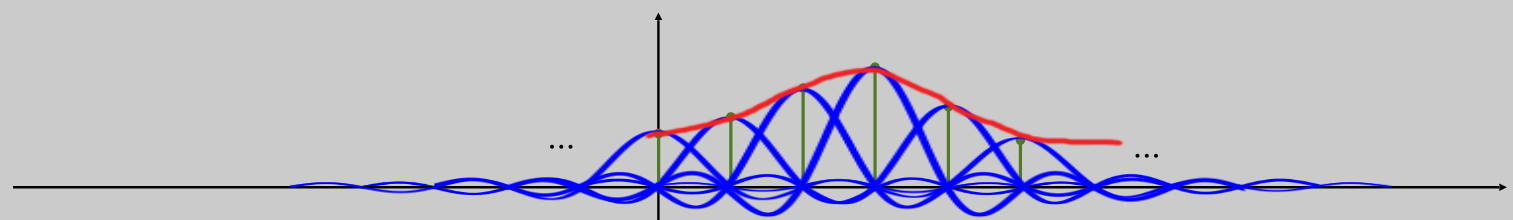
\includegraphics[width=\textwidth]{Screenshot_2020-11-15 Lecture11B - Lecture11B pdf.png}
\end{frame}

\end{document}
